\documentclass[a4paper,11pt]{report}
\usepackage[T1]{fontenc}
\usepackage[utf8]{inputenc}
\usepackage[english]{babel}
\usepackage{lmodern}
\usepackage{amsmath, systeme}
\usepackage{amsfonts}
\usepackage{amssymb}
\usepackage{amsthm}
\usepackage{graphicx}
\usepackage{color}
\usepackage{xcolor}
\usepackage{url}
\usepackage{theorem}
\usepackage{textcomp}
\usepackage{listings}
\usepackage{hyperref}
\usepackage{parskip}
\usepackage{svg}
\usepackage{epigraph}
\usepackage{amssymb}
\usepackage{graphicx}
\usepackage[ligature, inference]{semantic}
\usepackage{float}   % For H placement
\lstset{
	basicstyle=\ttfamily\small,  % Use a smaller monospace font
	lineskip=-2pt,               % Reduce the vertical space between lines
	breaklines=true              % Allow long lines to wrap
}

\usepackage{semantic}

\title{Project report for Languages, Compilers and Interpreters}
\author{Dario Bekic}
\date{\today}

\begin{document}

\maketitle
\tableofcontents

\begin{abstract}
This report includes the necessary design explanations for the A.Y. 2024/2025 project of the Languages, Compilers and Interpreters at Università di Pisa.
The full project can be found on GitHub visiting this \href{https://github.com/wuacs/unipi-lci/tree/main/project}{link}.
The project's main goal is to design and implement aspects of programming languages in OCaml. Three main languages were developed: MiniImp and Mini(ty)fun and MiniRISC. For \verb|minifun|, it was developed a typed version \verb|minityfun|. For those languages we first define their ASTs and evaluation functions, then, using OCamllex and Menhir we develop a lexer and a parser for those languages. The formal, ambiguous, grammars can be found \href{https://lceragioli.github.io/pages/Slides/semantics.pdf}{here} and \href{https://lceragioli.github.io/pages/Slides/types.pdf}{here} and the explanations of how the ambiguities were resolved is detailed in \autoref{chap:parsing}.
\end{abstract}

\section{MiniImp}\label{Section::MiniImp}

MiniImp was divided in two main modules: $\verb|miniimp.mli|$ which provides core functions to experiment with the language, and $\verb|miniimp_ast.mli|$ containing all the types which reify the language in OCaml.
In addition, for the lexing and parsing, modules $\verb|miniimp_lexer.mll|$ and $\verb|miniimp_parser.mly|$ were created. Together, the modules form a library named $\verb|miniimp|$, which can be used to parse and execute programs written in MiniImp.

\subsection{Parsing Conflicts}\label{Sec::parsingImp}

In the following sections we present the conflicts found when translating the \href{https://lceragioli.github.io/pages/Slides/semantics.pdf}{formal grammar of MiniImp} to an LR(1) grammar.

\subsubsection{While}

	One conflict flagged by Menhir is the following:
	\begin{lstlisting}[caption={Shift-reduce conflict with while term}, captionpos = b]
WHILE bool_expr DO command

Shifting: 

command . SEQ command

Reducing:

WHILE bool_expr DO command .

Lookahead symbol: SEQ
	\end{lstlisting}
	The shifting represents placing a sequence of commands in the body of the \verb|WHILE| construct.
	The reduce represents placing a \verb|;|, i.e. a \verb|SEQ| character, after a \verb|WHILE|, because the entire \verb|WHILE| expression could be reduced to a term.\\
	\textbf{Adopted disambiguation}: for a sequence of operations to take place in the body of a while construct we require the use of brackets. We create the non-terminal $\verb|block_command|$ representing either a sequence of instructions between brackets or an instruction which is interpreted as the whole body of the while(e.g. a new while construct or a single assignment).
	
\subsubsection{If}
	\begin{lstlisting}[caption={Shift-reduce conflict with if term}, captionpos=b]
Shifting: 
IF bool_expr THEN command ELSE command 
                               command . SEQ command

Reducing: 
IF bool_expr THEN command ELSE .
	\end{lstlisting}
	The shifting represents extending the \verb|ELSE|'s body with a sequence of commands
	The reduce represents executing first the \verb|IF| and then another command.\\
	\textbf{Adopted Disambiguation}: 
	Similarly to the problem above we need to be explicit how commands are grouped together in constructs which introduce a block. We decided that a sequence of instructions belongs to the nearest \verb|ELSE| block only if they are wrapped in brackets, otherwise only the first instruction belongs to the \verb|THEN| and the second is considered to be the next instruction happening after the nearest \verb|IF| block, i.e. $\verb|IF ... THEN ... ELSE c2 ; c1 | \equiv \verb|(IF ...); c1|$
	\subsubsection {Sequences}
	
	\begin{lstlisting}[caption={Conflict on the associativity of sequences}, captionpos=b]
Shifting:
command SEQ command 
command . SEQ command 

Reducing:
command SEQ command // lookahead token appears
command SEQ command .
	\end{lstlisting}
	
	The problem here is that we do not specify associativity for sequences of instructions.\\
	\textbf{Adopted Disambiguation}: we will give left associativity using the Menhir-specific directive:\\
	\verb|%left SEQ|(in \hyperref[Section::TyFun]{MiniTyFun}'s parser for completeness we instead reworked the grammar).
	
	\subsubsection {Operators}
	The following is another Shift-Reduce conflict: 
	
	\begin{lstlisting}[basicstyle=\small]
arit_expr MINUS arit_expr 
arit_expr . PLUS arit_expr // Looking Ahead at PLUS shift

arit_expr PLUS arit_expr
arit_expr MINUS arit_expr . // Looking Ahead at PLUS reduce
	\end{lstlisting}
	
	While having as a symbol of look-ahead \verb|PLUS|, we could be shifting
	or immediately reducing the \verb|MINUS| operation.\\
	\textbf{Adopted Disambiguation}: we will give left associativity to arithmetic(and boolean) tokens. The \verb|NOT| operator is given higher through Menhir ad-hoc semantics explained (\href{https://gallium.inria.fr/~fpottier/menhir/manual.pdf#subsubsection.4.1.4}{here}).


\section{MiniFun}
\label{Section::MiniFun}

MiniFun is a simple untyped functional language and all its implementation can be found in the $\verb|minifun.mli|$ module. A parser was not implemented for MiniFun but instead for its \hyperref[Section::TyFun]{typed counterpart}. \verb|minifun.mli| defines both the type representing the language abstract syntax tree and an $\verb|eval_fun_ast|$ which takes a value of type $\verb|ast|$, representing a program written in MiniFun, and returns an element of type $\verb|value|$ which can be either a function, since we are in a functional language, an integer or a boolean.
The run-time environment is typed $\verb|env|$ which is simply a map with strings as keys, so that we can keep track of variables. The environment is generic: we will be creating mappings for types, values and other variable-related information.
One interesting thing of the evaluation function is that, if it fails to resolve a variable during its execution, (i.e. said variable was not initialized with a $\verb|Let|$ or $\verb|LetFun|$ construct) it fails.


\section{Minityfun}\label{Section::TyFun}

MiniTyFun is a typed version of \hyperref[Section::MiniFun]{MiniFun}. 

\subsection{Missing Rules}

The only two rules which differ between MiniTyFun and MiniFun are the rules involving the typed constructs i.e. anonymous function declaration ($\verb|FUN|$) and the recursive function definition ($\verb|LET FUN|$).
\begin{figure}[H]
$\verb|LET FUN|$
\\
\[
\inference[]
{ 
	\Gamma[f \mapsto \tau] \vdash t' \triangleright \tau''\quad \tau = \lambda \texttt{->} \gamma \quad 
	\Gamma \vdash t \triangleright \gamma
}
{
	\begin{array}{c}
		\Gamma \vdash  \text{ letfun } f x:\tau = t \text{ in } t' \triangleright \tau''
	\end{array}
}
\]	
\end{figure}

$\verb|FUN|$
\\
\[
\inference[]
{ 
\Gamma \vdash t \triangleright \tau'
}
{
\begin{array}{c}
\Gamma \vdash  \text{ fun } x:\tau \texttt{ => } t \triangleright \tau \rightarrow \tau'
\end{array}
}
\]

\subsection{Type checking}

The type checking function works on the AST and keeps track of a type environment which consists of a mapping between each variable encountered during a left-traversal of the AST and a value which represents the possible types a variable can have:
$\verb|Integer_t|$ for integers, $\verb|Boolean_t|$  and $\verb|Closure_t(d, c)|$ for booleans and functions respectively. The evaluation of a node in the AST returns its type after recursively invoking the type checking function on its children with an updated context. The update to the environment depends on the node: for example, recursive functions which are typed $f \;x : \tau \mapsto \tau'$ introduce the binding of the parameter $x$ in the body of the function with type $\tau$ and introduce $f$ with type $\tau \mapsto \tau'$, since it is a valid identifier in the body of the recursive function.

\subsection{Parsing Conflicts}

Now we show a list of conflicts found when translating the ambiguous grammar of MiniTyFun in an LR(1) equivalent and the adopted disambiguation.
Shared conflicts which have already been discussed in \hyperref[Sec::parsingImp]{MiniImp's section} are not re-reported as their solution is the same.

\subsubsection{LET/LETFUN}
	An example of operator precedence problem is the following:
	\begin{lstlisting}

term PLUS term // lookahead token appears
LETFUN VAR VAR TYPE_SEP typing term IN term . 

LETFUN VAR VAR TYPE_SEP typing term IN term 
term . PLUS term 
	\end{lstlisting}
	 We want the following \verb|... IN term PLUS term| to mean that in the context of \verb|LETFUN| (or \verb|LET|) we have the sum of two terms, not that we sum the \verb|LETFUN| term with another term. The issue this conflict indicates is that of operator precedence: we do not know whether we should reduce the term to the sum or to continue shifting. \\
	\textbf{Adopted Disambiguation}: \\
	First, we make a distinction between general context-introducing terms and applications, creating the non-terminal $\verb|basic_term|$ which is used in places where a literal or a variable is expected. To preserve the semantics of the language and to keep it readable we require brackets when using a context-introducing term instead of a literal or variable in applications: i.e. the following syntax is the one which gives the expected result: $\verb|f (LETFUN ... IN ...)|$. \\
	Then, we make the application left-associative making the correspondent production left-recursive. 
	For operators we decided to give priority to multiplication over addition(and subtraction): instead of using ad-hoc Menhir mechanisms we re-worked the grammar by distinguishing between operations with inferior level of precedence ($\verb|additive_expr|$) and an higher one ($\verb|multiplicative_expr|$).
	
\subsubsection{Application}


We make application left-associative by creating a left recursive rule \\$\verb|operation = operation literal|$.
This means that the double application $\verb|t t' t''|$ is parsed as $\verb|(t t') t''|$. We use $\verb|literal|$ because we make the decision that other terms are required to be enclosed in brackets; this means that, for example, \verb|f - 4| will be interpreted as the difference between identifier $\verb|f|$ and the integer 4. However, \verb|f (-4)| is the application of \verb|-4| to the identifier \verb|f|. 

\section{Control-Flow Graphs}\label{Section::CFG}


\subsection{Almost Maximal Block CFG}
Our control-flow graphs follow a variation of the Maximal Block approach.
Our CFG-building function for \hyperref[Section::MiniImp]{MiniImp} maintains the invariant that the initial node(called $\verb|entry|$) of any sub-CFG shall not have any incoming arc and the last(called $\verb|exit|$) shall not have any outgoing arc.
Consider the MiniImp program in listing \ref{lst:fiboImp}. The CFG, rendered by using the file produced by function \ref{HTU::Dot::impCfg}, using the \href{https://graphviz.org/download/}{graphiz} package, can be seen in figure \ref{fig:cfg:fibonacci}.
Notice how there are 2 $\verb|SKIP|$ nodes which could be merged, but they are kept separate for the following 2 reasons:
\begin{enumerate}
  \item Each $\verb|while|$ construct generates a new $\verb|exit|$ node because the end node must not have any outgoing arc, this is the node $Q$ in our figure. The sub-CFG created by parsing the while node consists of nodes $I, P, Q$.
  \item Each $\verb|if|$ construct generates a final block where the two sub-CFGs represented by its branches will merge into. Since it does not know the structure of the CFG corresponding to its branches it cannot merge its final nodes. One would need to check that at least one of its branches is made of only $\verb|Nop|$ instructions and then could merge them. This check would need to be made for each construct which merges nodes.
 \end{enumerate}
Sequences of blocks are correctly compacted in one block: in the initial block $X$, the first two instructions of the \verb|main|, which in terms of MiniImp's AST are a sequence of instructions, have been compacted together with the guard generated by the $\verb|if|$ node.

\begin{lstlisting}[caption={N-th Fibonacci number in MiniImp}, captionpos=b, label={lst:fiboImp}]
    def main with input in output out as
        x := in;
        out := 0;
        if not x < 2 then (
            out := 0;
            second := 1;
            while not x < 2 do (
                temp := out;
                out := out + second;
                x := x - 1;
                second := temp
            )
        )
        else (
            out := 0
        )
\end{lstlisting}


\subsection{MiniImp CFG to MiniRISC CFG}

The translation traverses the MiniImp control-flow graph in post-order: when translating a MiniImp simple instruction $x$ we recursively translate sub-expressions of $x$ by providing them with a register $r$ where their result must be written, then $x$ can refer to the sub-expression result through $r$ (and translate other sub-expressions by calling them with register $r+1$).

\subsubsection{Translating expressions}

In MiniImp we may have the instruction $\verb|x := e|$ where $e$ is either a boolean or an arithmetic expression. Each sub-expression of $e$(i.e. a multiplication, an \textit{and} operation ecc.) which contains a constant in one, of its at most two operands, is translated to its constant MiniRISC counterpart ($\verb|mulI, andI, ...|$) through the generic function $\verb|convert_minirisc_bop|$ which is used both to translate boolean expression and arithmetic expressions and perform the post-order traversal.

\begin{center}
	\begin{figure}
	  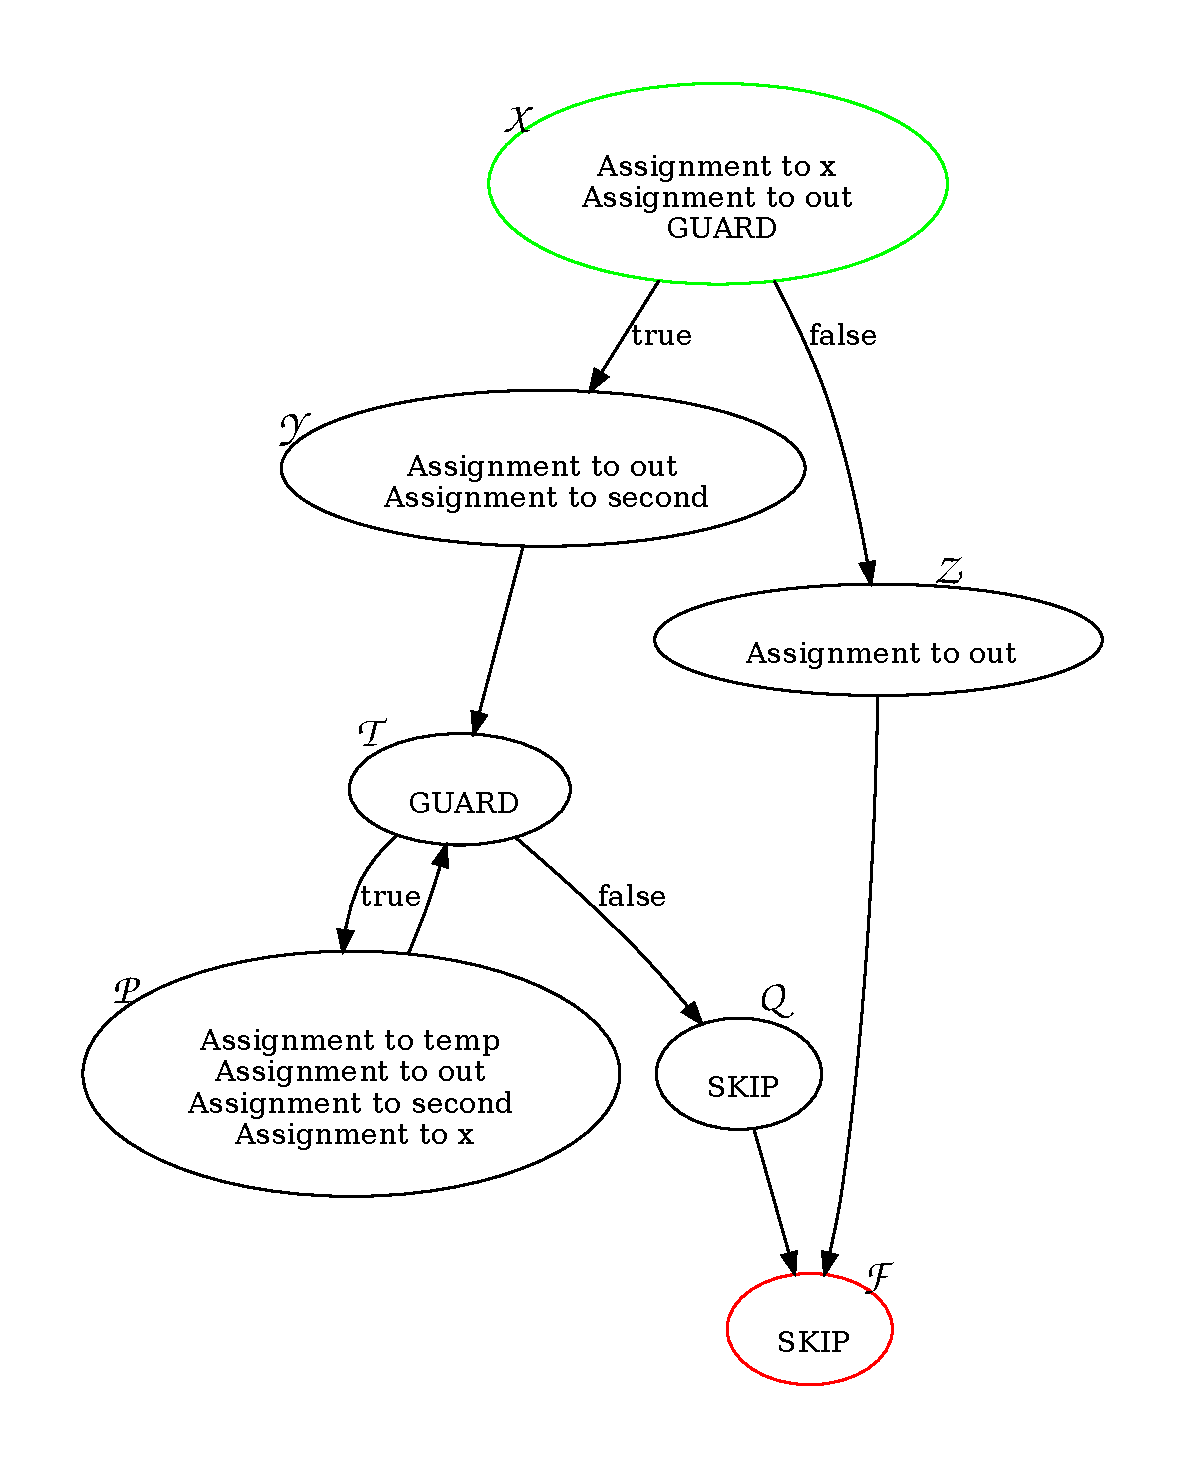
\includegraphics[width=\linewidth]{./report_resources/cfgimpfibo.pdf}
	  
	  \caption{\label{fig:cfg:fibonacci} CFG for Fibonacci's program}
\end{figure}
\end{center}



\section{Static Analyses}

We implemented two data flow analyses for the Intermediate Representation of MiniRISC: the defined variable analysis, implemented by the module $\verb|defined_analysis|$ and the liveness analysis implemented by the \\$\verb|liveness_analysis|$ module.
We defined utility functions on the Control Flow Graph which may be used by different data flow analyses, such as $\verb|get_bottom|$ which returns the set of all registers defined in our Control Flow Graph, which is used, for example, when initializing the $\verb|LIVE_IN and LIVE_OUT|$ sets at the start of the liveness analysis.


\subsection{Non-minimal CFG}

As explained in the \hyperref[Section::CFG]{CFG} section we used maximal blocks. This means that we need to specify what is a \textbf{used} register in a block and what is a \textbf{defined} register in a block. In a minimal block CFG each block $x$ contains only one instruction, which implies that the set \textbf{used}($x$) are the registers at the right-hand side of the instruction while the \textbf{defined} registers are at the left-hand side. 
In our setting, \textbf{used}($x$) contains the registers which appear on the right-hand side of a MiniRISC instruction $y$, and never appear on the left-hand side of an instruction in instructions happening before $y$.
Our function, $\verb|used_registers|$, in the $\verb|data_flow_utils|$ module achieves this, returning a set of used registers in the given block.
The \textbf{defined} register set instead is the set of all registers which appear on the right-hand side of an instruction in a block.

\section{MiniRISC}\label{Section::MiniRISC}


For MiniRISC we decided to split the code between modules $\verb|minirisc.mli|$ which provides the types for instructions and support data structures (like Maps and Sets for registers, memory addresses...) which are part of the environment needed for compiling and/or interpreting MiniRISC code.
The MiniRISC compiler is implemented by module $\verb|target_code.mli|$ which exposes types and functions which can help customize the compiling process. The $\verb|spill_metric|$ type,  for example, can make the compiler choose a different focus in its register allocation phase than what is used normally (by default the value $\verb|cost_metric|$, defined at module level, is used).
Of course, there is the function $\verb|generate_target_code|$ which simply outputs the object code to a file; the function takes optional arguments as described here.
MiniRISC instruction's type was divided between simple instructions (called $\verb|scomm|$) and instructions (called $\verb|comm|$). The first are used in the IR of the MiniRISC program and can be later on reified easily when generating the target code.

\subsection{Registers and Labels}
A register identifier is an integer and special integers, like the input register and output register, are given reserved integer identifiers, see \href{https://github.com/wuacs/unipi-lci/blob/a630eb254e4eadffe7290cbda91d80f921402fde/project/src/lib/minirisc.mli#L28}{here}.
The type label, i.e. an instruction identifier to which a jump instruction can refer to, is an integer too. In the generation of the MiniRISC code, however, we substitute the initial label with the $\verb|main|$ label as per the specification. Note that we do not have to change any jump instruction as the invariant we keep for our intermediate representations assures no jumps to initial blocks, and thus no jump to to the main label can be found in any instruction.
\subsection{Handling guards}

Guards modify the control-flow of our program, i.e. they represent conditional $\verb|jump|$ instructions. We adopt the convention that the written register of the last instruction contains the boolean which the $\verb|cjump|$ instruction will check. 

\subsection{Optimization}

For the optimization regarding the number of used registers in the generated code we decided to use the Chaitin-Briggs algorithm which can be found in the $\verb|target_code|$ module. The algorithm is parametric in the spill metric, however, our translation function $\verb|translate_cfg_to_target|$ uses a simple cost metric which counts the times a register has been read or written to.
Note that any spill metric should be a \textit{lower is better} metric as the algorithm picks the lowest w.r.t the metric among the uncolored registers to spill.

\subsubsection{Handling special registers}

The coloring algorithm may map the input/output register to either memory or to a different register. However, the interpretation of MiniRISC target code happens by initializing the input register with an appropriate value and the output is derived by reading the output register. Our coloring algorithm then needs to return not only the IR with the compressed registers, but also 2 memory locations (of type $\verb|memory_loc|$) which represent the memory location after coloring of the input and output registers. We may then add instructions which move the value out of the input register to its colored counterpart and append instructions which move the value in the colored counterpart of the output register to the output register as the last instructions of the final block.

\subsection{Translating the CFG to ordered code}

The translation of the MiniRISC Control-Flow Graph is done in a single depth-first traversal of the graph. This implies that the final block's code is not necessarily the last block in the generated code. This is why we define a reserved label $\verb|exit_label|$ to which a new unconditional jump appended to the generated code of the CFG's final block will jump to, and the exit label is added to an artificial last instruction which does nothing. This implementation would allow us to incorporate $\verb|return|$ statements in the language easily by jumping to the \href{https://github.com/wuacs/unipi-lci/blob/a630eb254e4eadffe7290cbda91d80f921402fde/project/src/lib/target_code.ml#L15}{exit label}.

\section{How to use}

The objective of the laboratory was to design and implement the following components:

\begin{itemize}
	\item A MiniFun interpreter 
	\item A MiniTyFun interpeter and parser
	\item A MiniImp interpreter and parser
	\item A MiniImp compiler to MiniRISC which needs to provide two options: one for optimizing the number of registers used in the generated code, and one for performing a static analysis to check whether every variable was initialized before use. 
\end{itemize}

We additionally implemented an executable for testing the static analyses and one which provides produces \href{https://en.wikipedia.org/wiki/DOT_(graph_description_language)}{Dot} compliant files to display visually the result of the most important operations implemented on the \hyperref[Section::CFG]{Control Flow Graph}.
The following sections explain how to test each component.
Note that every executable is in the $\verb|bin/|$ folder and can be used by $\verb|dune exec filename ...|$ where $\verb|...|$ is one or more parameters with the semantics explained in the following sections.

\subsection{MiniFun interpreter}

We did not implement a Parser for MiniFun, instead we did it for its typed counterpart, as such the only way to customize the interpretation a MiniFun program is to modify the $\verb|staticly_evaluated|$ identifier defined at top of the module $\verb|./bin/untyfun.ml|$ and specify an AST value of the corresponding type whose definition can be found $\verb|./lib/minifun.mli|$. 
To execute the minifun program to evaluate the \verb|staticly_evaluated| identifier use:
$$
\verb|dune exec untyfun static|
$$

\subsection{MiniTyFun}

For MiniTyFun the following command can be used to evaluate a program with filepath named $x$ and output its result on stdout:
$$
\verb|dune exec tyfun interpret_file x|
$$

\subsection{MiniImp}

For MiniImp you can use the following command to execute a MiniImp program with a file path $x$.

$$
\verb|dune exec imp execute x|
$$

\subsection{Target Code}

For MiniRISC we provide a compiler of MiniImp programs which has 2 optional arguments.
\begin{itemize}
	\item \textbf{registers=x} sets the number of assumed registers in the MiniRISC code to \textbf{x}. If this argument is missing \textbf{x} is set to 4.
	\item \textbf{undefined\_check} the compilation performs a static analysis to check for potential undefined variables. If such a variable is found, the process fails. If this argument is missing then no check is made.
\end{itemize}

The command to execute the compiler is
$$
\verb|dune exec target build x y [registers=k] [check_undefined]|
$$

Where square brackets indicate possible omission and $x$ and $y$ are respectively the file paths of the input file containing the MiniImp program and the output file where the MiniRISC code needs to be written to.

We additionally provide an interpreter, which is a simple wrapper around the compiler which, after compilation, executes the produced code. No parser was created so this was the main testing function.

To use the interpreter execute the following command

$$
\verb|dune exec target eval x y|
$$

where $x$ is the input file path and $y$ is the integer given as input to the MiniImp program.

\subsection{Dot graphs}

To render visually data structures particularly important, like Control-flow graphs, or the result of applying optimization techniques on the CFG of MiniRISC programs we relied on the \href{https://en.wikipedia.org/wiki/DOT_(graph_description_language)}{Dot} language. All those functions are testable through the executable $\verb|dot.ml|$ and any file produced can then be rendered using the \href{https://graphviz.org/}{Graphviz} package. As an example, to render a dot file to a PDF:
$$
\verb|dot -Tpdf file_name -o file_output|
$$

where $\verb|file_name|$ is the file path of one of the files produced by one of the executable's functions and $\verb|file_output|$ is the file path of produced PDF file.

To generate DOT files representing various aspects of a MiniImp program or its translation to MiniRISC, the following commands are available:

\begin{enumerate}
	\item \label{HTU::Dot::impCfg} \textbf{Control Flow Graph (CFG) of a MiniImp program:}
	
	To generate a DOT file containing the control flow graph of a MiniImp program, run the command:
	
	\begin{verbatim}
		dune exec dot miniimp input_file output_file
	\end{verbatim}
	
	\item \textbf{Control Flow Graph (CFG) of the equivalent MiniRISC program:}
	
	To generate a DOT file containing the control flow graph of the MiniRISC program equivalent to a MiniImp input program, run the command:
	
	\begin{verbatim}
		dune exec dot minirisc input_file output_file
	\end{verbatim}
	
	\item \textbf{Interference graph of an unoptimized translation:}
	
	To generate a DOT file showing the interference graph of an unoptimized translation of a MiniImp program to MiniRISC, run the command:
	
	\begin{verbatim}
		dune exec dot interference input_file output_file
	\end{verbatim}
	
	\item \textbf{Control Flow Graph of an optimized translation:}
	
	To generate a DOT file showing the control flow graph of an optimized translation of a MiniImp program to MiniRISC for a target architecture with at most \texttt{registers} registers, run the command:
	
	\begin{verbatim}
		dune exec dot optimized input_file_path output_file_path registers
	\end{verbatim}
	
	\item \textbf{Control Flow Graph with liveness information:}
	
	To generate a DOT file representing the control flow graph of a MiniImp program translated to MiniRISC, where each node contains the set of registers \textit{live in} and \textit{live out}, run the command:
	
	\begin{verbatim}
		dune exec dot liveness input_file_path output_file_path
	\end{verbatim}
	
	\item \textbf{Control Flow Graph with undefinedness information:}
	
	To generate a DOT file representing the control flow graph of a MiniImp program translated to MiniRISC, where each node contains the set of registers certainly defined at the start and after the block, run the command:
	
	\begin{verbatim}
		dune exec dot undefinedness input_file_path output_file_path
	\end{verbatim}
\end{enumerate}

\texttt{input\_file} and \texttt{input\_file\_path} represent the path to the input file containing the MiniImp program.
\texttt{output\_file} and \texttt{output\_file\_path} represent the path to the output file where the generated DOT file will be written.
\texttt{registers} is an optional parameter specifying the maximum number of registers available for optimization.


\end{document}

